\setstretch{2}
\section{Outline / Bullet Points}


\subsection{Results}

\begin{itemize}
    \item While a high quality image could be formed on the sCMOs camera which clearly shows the vascular structure of the retina could be formed - albeit polluted by glare in the centre of the vision. A sufficient image could not be formed on the FLIMera but there is sufficient signal to attempt SFLIM unmixing. This could be due to the low fluorescence contrast as evidenced by the fluorescence intensity image recorded with a lp500 filter in the SCMOs camera. 
    \item Can't map FAD across the retina but can use the signal to extract a general trend in the FAD concentration wrt oxygenation.
    \item In the histograms recorded by the FLIMera there was also the addition Gaussian like thermal noise characteristic that was ultimately corrected by simply neglecting these values in the calculation of the cost function of the minimisation process (phi). While this does decrease the overall energy in the signal what is left should be capable of capturing both the long and short lifetime dynamics.
    \item A brief comparison of the possible dark field correction methods yielded no significant change in the recovered concentration of retinal FAD  - dark-field correction by fitting a modified Gaussian to the artefact and subtracting from each histogram, masking the effected time bins, and simple fitting through the artefact.
\end{itemize}


\section{FAD as a marker of retinal health}
Mapping the concentration of FAD would enable diagnosis at the initial stages of retinal disease where metabolic function is compromised - before a patient would present with permanent physical damage to vision. FAD is produced throughout the body as a by-product of metabolisation of oxygen to create ATP - the bodies source of energy - through aerobic respiration(\cref{eq:resp})~\cite{berg2007biochemistry}. In detecting retinal disease, the retina would exhibit abnormal metabolic activity - ATP usage - and would be detectable as corresponding areas with abnormal FAD concentrations. 
\begin{equation}\label{eq:resp}
    \ce{C6H12O6 + 6O2 -> 6CO2 + 6H2O + ATP}
\end{equation}
While the changes in retinal FAD distribution associated with retina disease is not know the feasibly of detecting changes in FAD can be appraised in animal models using the SFLIO device and SFLIM unmixing technique developed in this thesis. The consumption of systemic oxygen can be restricted to artificially lower FAD concentration. At normoxic conditions (\SI{21}{\percent}\ce{FiO2} oxygen metabolism is typical however in hypoxic conditions (\SI{15}{\percent}\ce{FiO2}) the retina is starved of oxygen thus lowering the detectable concentration of FAD. After death when all metabolic processes have cease the concentration of FAD should tend to zero - in rat cortexes this has been reported as the FAD leaking out of arteries forming `halos'~\cite{martinez2017understanding}.
In this chapter, the SFLIO device (described in \cref{chap:fliodevice}) was used to record \textit{in-vivo} SFLIM images of the retinas of anaesthetised rats under normoxic, hypoxic, and post-mortem conditions where the concentration of retinal FAD is recovered using the SFLIM unmixing algorithm (described in \cref{chap:tensSFLIM}). Successful detection of FAD is then signified by the changes in the recovered retinal FAD concentration being compatible with what is expected with aerobic respiration. Finally, from this a feasibility of quantifying retinal FAD in human retinas can explored.


\section{\textit{In-vivo} Rat Imaging Protocol}\label{sec:expprotocol}
The imaging experiments were carried out in the labs of Prof. Kenneth J. Smith (Institute of Neuroinflammation, UCL) where Helen Yang (Institute of Neuroinflammation, UCL) prepared the rats for imaging, administered isoflurane to aenisthitise them, and monitored general health throughout the imaging session. An external nitrogen supply was mixed with room-air and fed into a fitted nosecone to control the fraction of inspired oxygen. Albino rats were chosen for their lack of melanin in the eye which reduces the loss of emitted retinal autofluorescence to absorption and maximising SNR in detected fluorescence. As shown in~\cref{fig:ratsetup}, the rat is secured to the imaging platform and the pupil is dilated using Tropicamide drops to increase pupil diameter (\qtyrange{1.20}{4.35}{\mm}~\cite{himmel2019pupillary}) - maximising the number of detected photons. The eye lids are fixed open with stitches and contact lens is fitted to index-match the rats eye lens. Viscotears gel is applied around the cornea to prevent it becoming dry and irritated causing additional eye movement and motion requiring correction. To accommodate the rats smaller eyeball diameter, of \SI{6.3}{\mm}~\cite{pazos2015rat}, a field-lens ($\varphi = 2''$, $f = \SI{85}{\mm}$) is fitted to the objective lens of the fundus camera. This additional lens did induce reflections from the illumination source off the front surface of the objective lens and rear surface of the field lens degrading some of the brightfield images with glare (\cref{fig:Ratscmosimages}a although careful positioning of the rat could remove them. This glare was observed to be independent of the motion of the retina which would cause errors in the detected motion in the phase-cross correlation process. Masking the affected area mitigates this. Alternatively, the glare could be removed using an image recorded of a non-reflective scene containing only the glare ($I_{dark}$) and linearly subtracting it from an recorded image ($I_{raw}$) to produce a glare-free image ($I$).
\begin{equation}\label{eq:glarecal}
    I = I_{raw} - \alpha I_{dark}
\end{equation}


\begin{figure}
    \centering
    \begin{annotatedFigure}{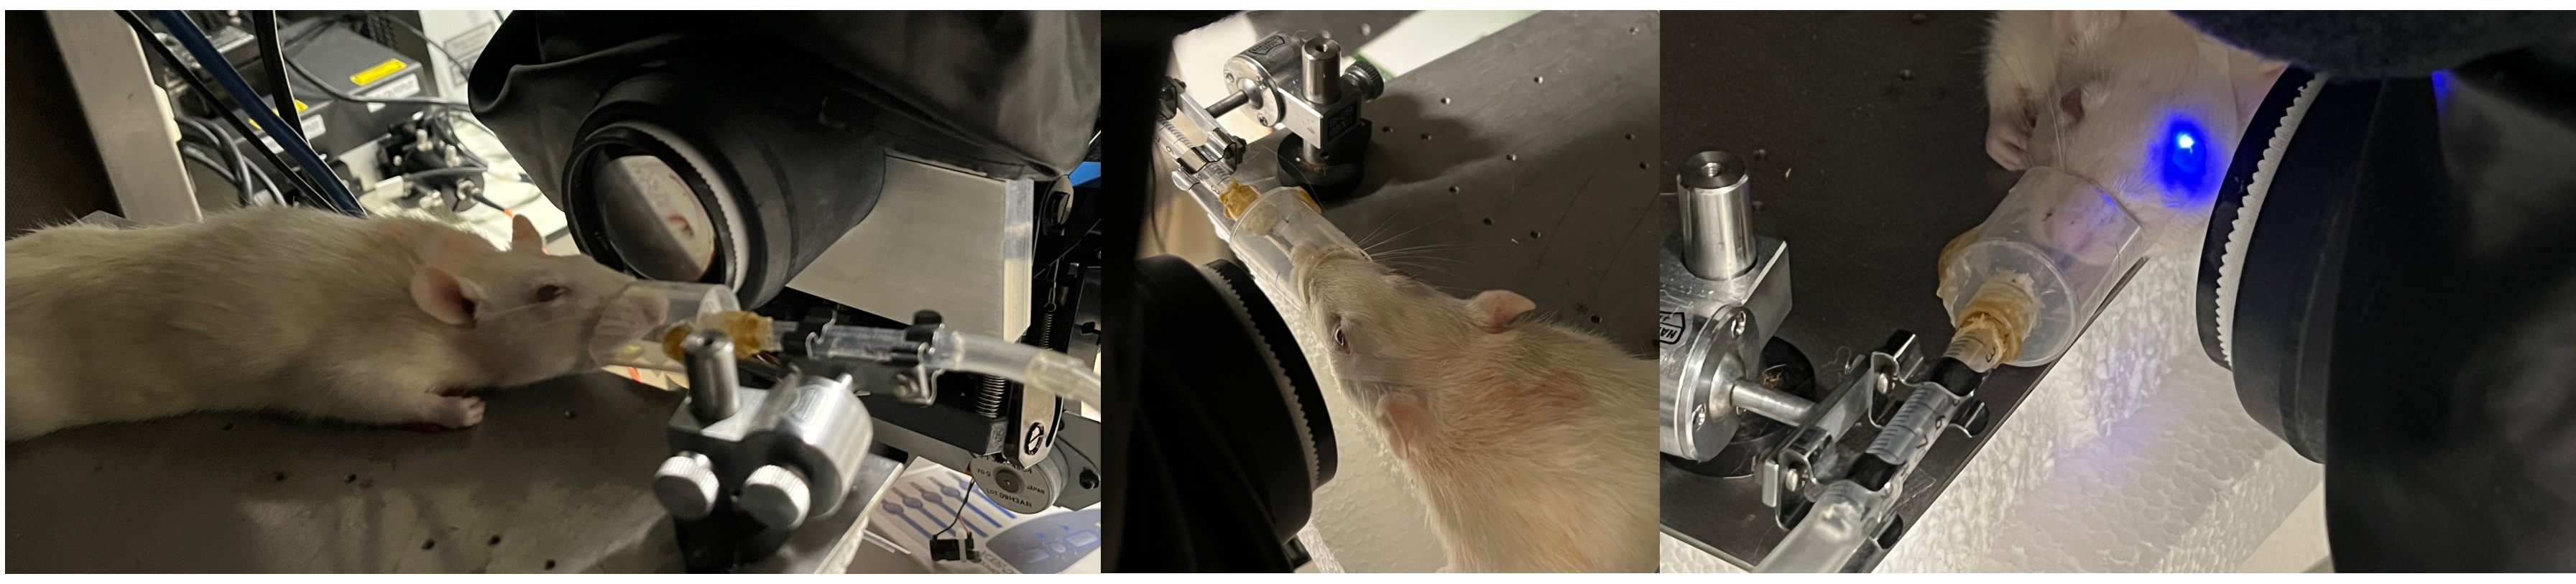
\includegraphics[width = \textwidth]{figures/ratUCL/RatSetupFigure.pdf}}
        \annotatedFigureText{0.015,0.83}{white}{0.3}{a)}
        \annotatedFigureText{0.435,0.83}{white}{0.3}{b)}
        \annotatedFigureText{0.66,0.83}{white}{0.3}{c)}
    \end{annotatedFigure}
    
    \caption{a) and b) The anaesthetised rat is positioned on the imaging platform perpendicular to the SFLIO system to have the rat's retina parallel with the image plane. The fundus camera is moved axially such that the illumination forms a focussed spot on the cornea - evenly illuminating the retina (c).}
    \label{fig:ratsetup}
\end{figure}
Two rats were images over three days. For each acquisition brightfield images are recorded continuously (\SI{50}{\ms} exposure at \SI{10}{\Hz}) in tandem with the FLIMera operating in raw mode over a two minute acquisition period for all 4 spectral filters. Due to the large file size generated from the FLIMera RAW acquiisition around \SI{10}{\minute} is required the build and save the \SI{50}{\giga\byte} stream of photon counts for each spectral channel. This SFLIM acquisition is carried out while the rats are cycled from normoxia to hypoxia (\SI{15}{\percent}\ce{FiO2}) and then back to normoxia again with an $\approx 5$~minute interval between each acquisition. These intervals between spectral filters and oxygenation states minimises any photobleaching and should ensure that metabolic processes and FAD concentration re-stabilise although long periods of hypoxia can cause the rat to die due to oxidative stress. SFLIM images were recorded for the first rat on the second day. As before (\cref{fig:flimerascmossync}), the two detectors are synchronised in time by initially having the laser shutter closed at the start of the acquisition and then opening it after a short period of time and detecting the Heaviside-like change in photon flux. Due to the anaesthetic the nervous response in the rats is suppressed which eliminates any visible saccades in the image sequence. The motion correction algorithm developed in \cref{chap:motionreg} is still utilised to ensure any small movements of the rat over the hour long imaging sessions does not cause misalignment between spectral filters. However due to the no pixel super-sampling was performed (\cref{fig:FLIMerareg}c).


\begin{figure}
    \centering
    \begin{annotatedFigure}{\includegraphics[width = \textwidth]{figures/ratUCL/RatsCMOSfigure.pdf}}
        \annotatedFigureText{0.025,0.91}{white}{0.3}{a)}
        \annotatedFigureText{0.35,0.91}{white}{0.3}{b)}
        \annotatedFigureText{0.68,0.91}{white}{0.3}{c)}
        \annotatedFigureText{0.19,0.425}{white}{0.3}{d)}
        \annotatedFigureText{0.52,0.425}{white}{0.3}{e)}
    \end{annotatedFigure}
    \caption{a - c) Shows example brightfield images recorded of each of the 3 rats imaged. Each frame is recorded over an integration time of \SI{30}{\ms} at a rate of \SI{10}{\Hz} where a small amount of glare is present in the highlighted region of a). In d) and e) a fluorescence intensity image was recorded using a \SI{500}{\nm} long-pass filter over integration times of \SI{1}{\second} and \SI{5}{\second} respectively.}
    \label{fig:Ratscmosimages}
\end{figure}

For the next three sections, \cref{sec:rat1day1results,sec:rat1day2results,sec:rat2results} the results will be presented separately and then brought together for a final meta-analysis and appraisal of the feasibility of detecting FAD in \textit{in-vivo} human retinas
\section{Results For Rat 1}\label{sec:rat1day1results}

\begin{figure}
    \centering

    \begin{annotatedFigure}{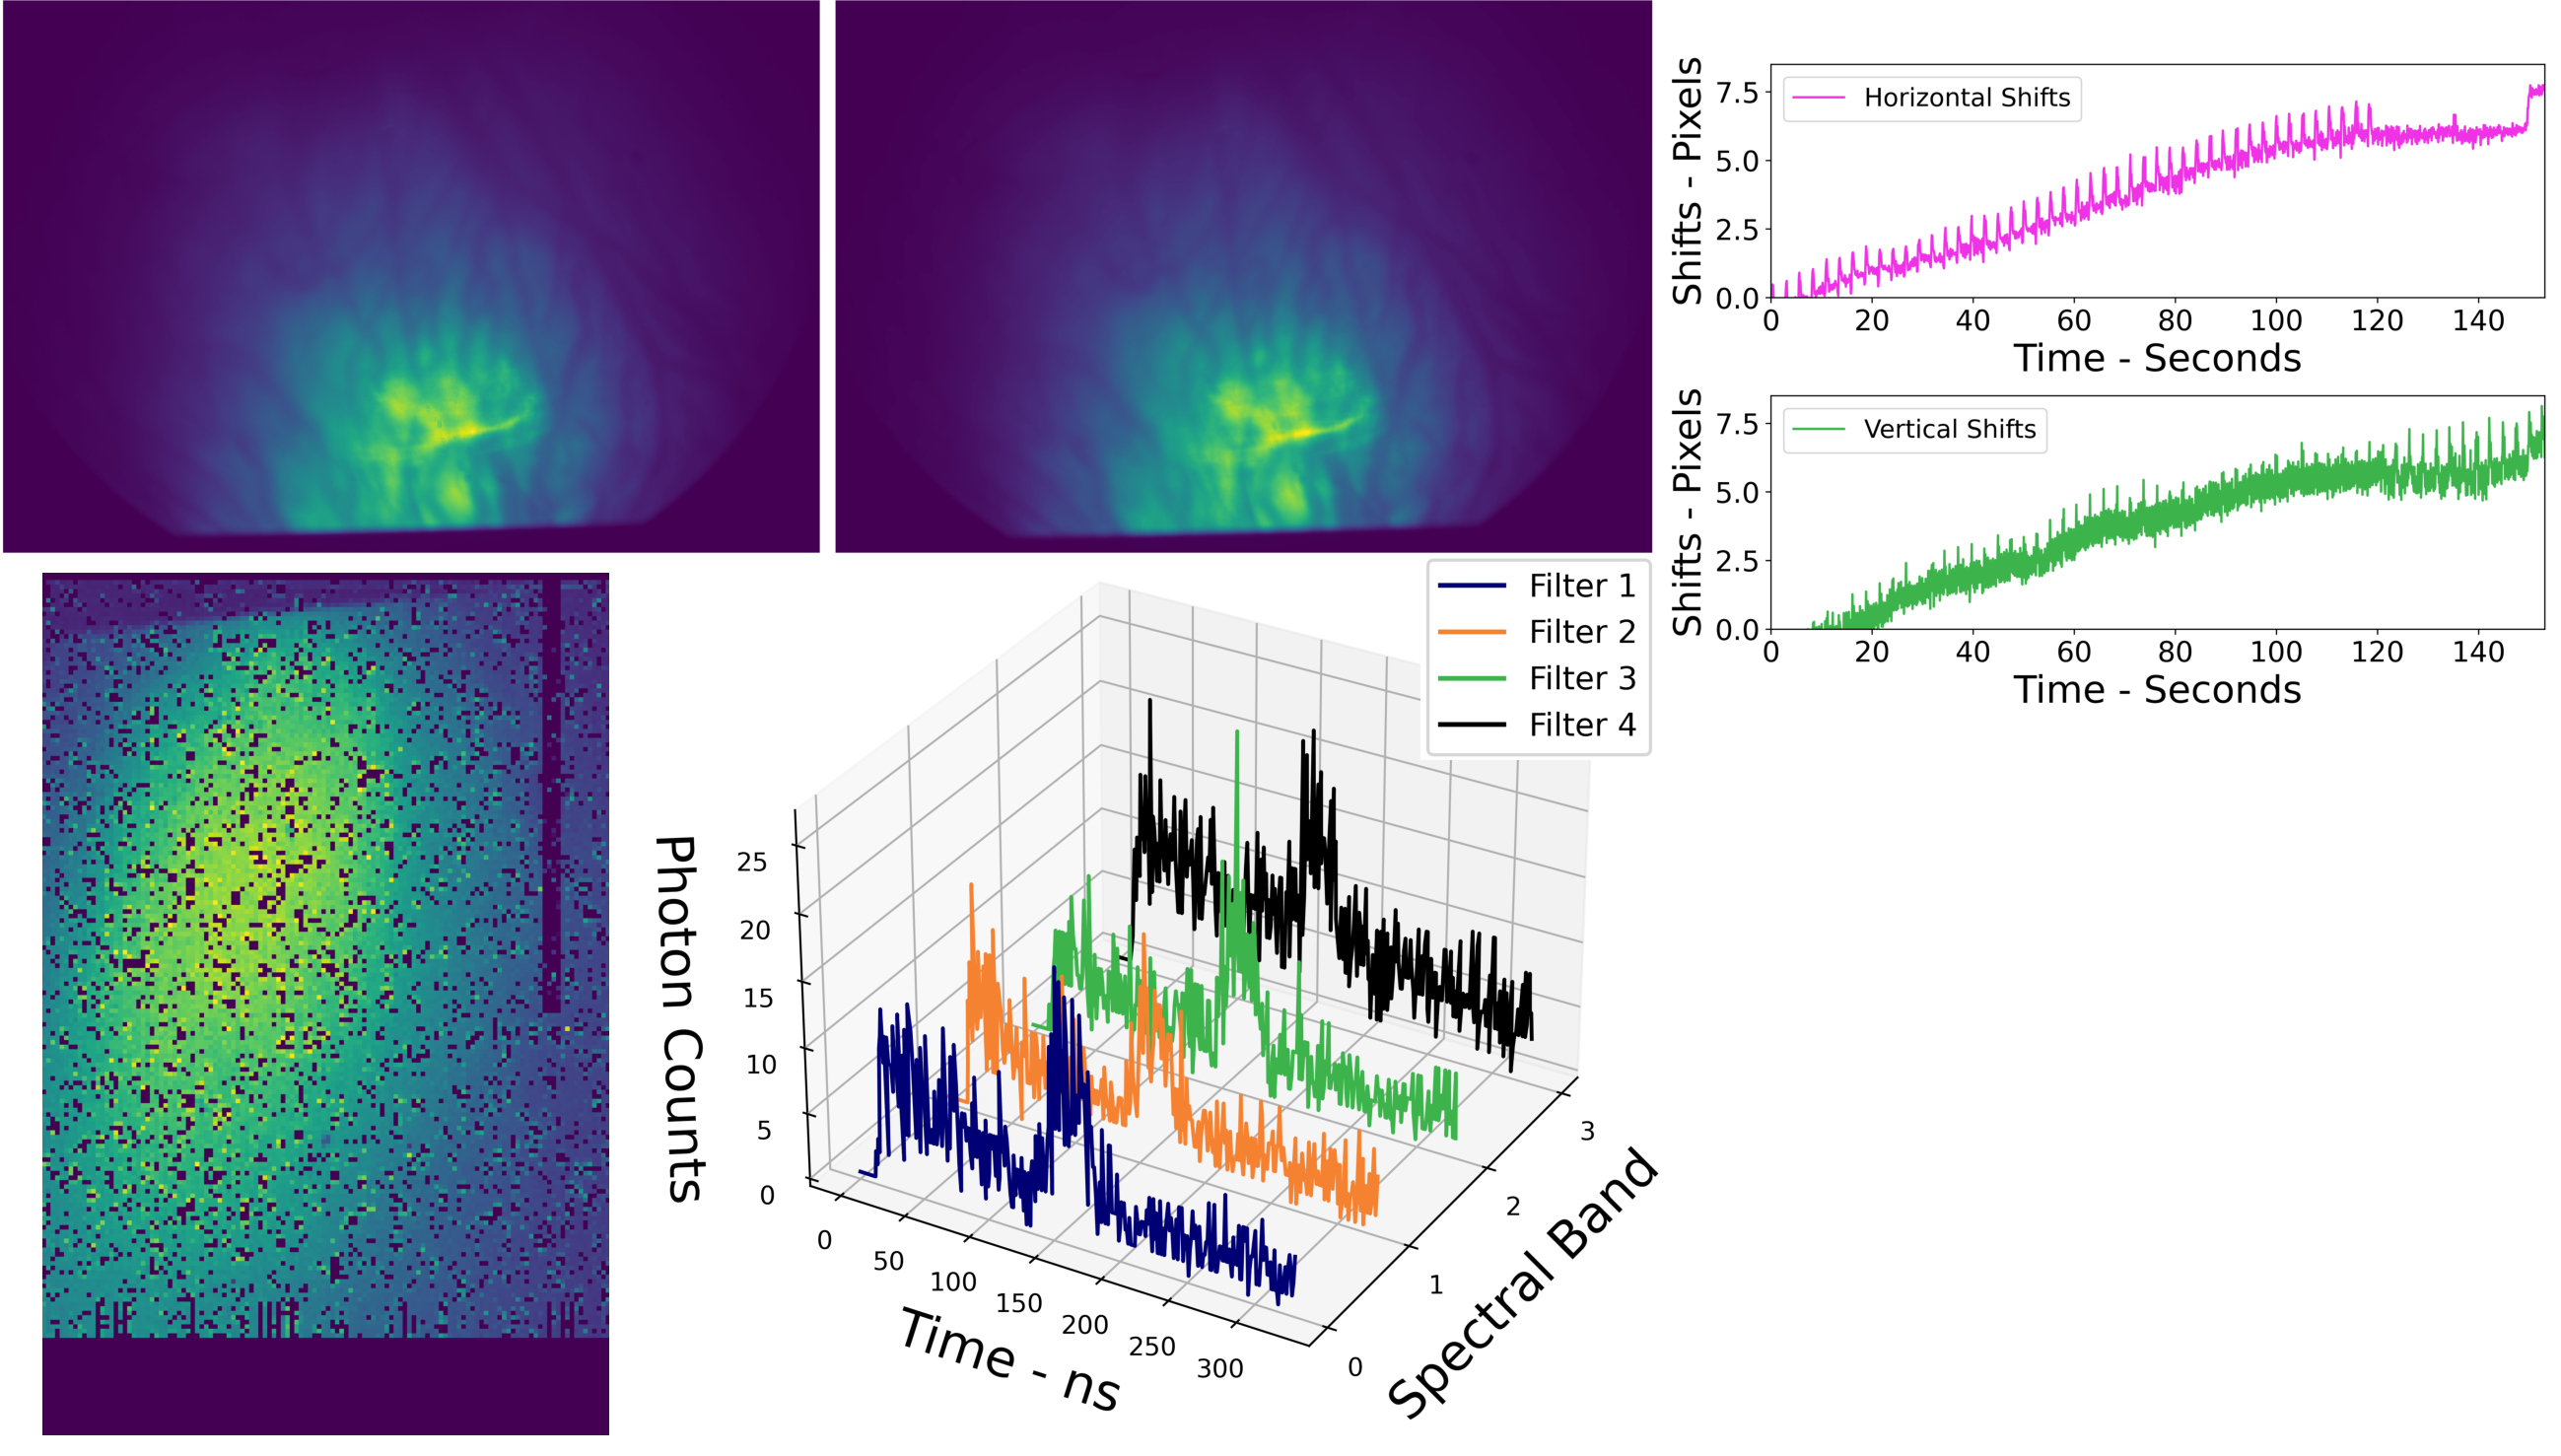
\includegraphics[width = \textwidth]{figures/ratUCL/ThesisFigure-Rat1RawData.pdf}}
    \annotatedFigureText{0.01,0.945}{white}{0.3}{a)}
    \annotatedFigureText{0.335,0.945}{white}{0.3}{b)}
    \annotatedFigureText{0.665,0.945}{black}{0.3}{c)}
    \annotatedFigureText{0.025,0.545}{white}{0.3}{d)}
    \annotatedFigureText{0.3,0.55}{black}{0.3}{e)}
    \end{annotatedFigure}
    
    \caption{Caption}
    \label{fig:rat1rawdata}
\end{figure}

\subsection{Darkfield Correction}
In the histo

\section{Results For Rat 1, Day 2}\label{sec:rat1day2results}

\section{Results For Rat 2}\label{sec:rat2results}

\section{Summary Of Results}

